\begin{enumerate}[label=\thesection.\arabic*.,ref=\thesection.\theenumi]
\numberwithin{equation}{enumi}
\item Sketch the direct polar plot for a unity feedback system with open loop transfer function
\begin{align}
\label{eq:ee18btech11002_gain}
G(s) = \frac{1}{s(1+s)^2}
\end{align}
\\
\solution  
The polar plot is obtained by plotting $\brak{r,\phi}$
\begin{align}
r&=|H(\j\omega)||G(\j\omega)|
\\
\phi&=\angle H(\j\omega)G(\j\omega), 0 < \omega < \infty
\end{align}
The following code plots the polar plot in Fig. \ref{fig:ee18btech11002polar_plot}

\begin{lstlisting}
codes/ee18btech11002/polarplot.py
\end{lstlisting}
\begin{figure}[!ht]
\centering
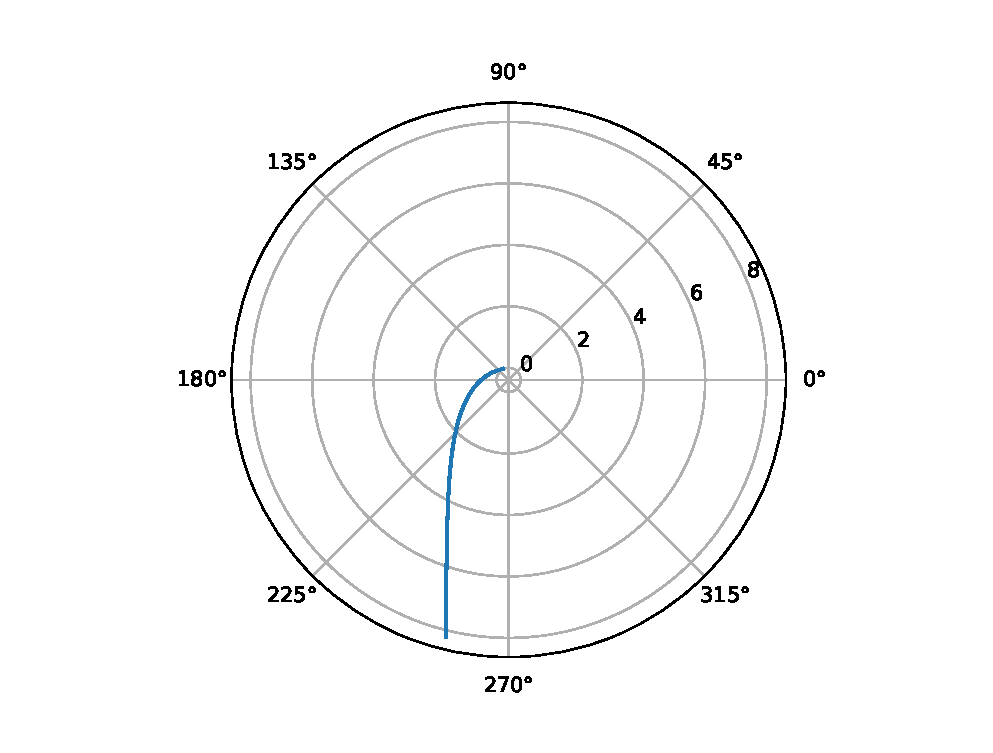
\includegraphics[width=\columnwidth]{./figs/ee18btech11002/ee18btech11002.eps}
\caption{Polar Plot}
\label{fig:ee18btech11002polar_plot}
\end{figure}
\item Sketch the inverse polar plot for \eqref{eq:ee18btech11002_gain}
\\
\solution The above code plots the polar plot in Fig. \ref{fig:ee18btech11002inverse_polar_plot} by plotting  $\brak{\frac{1}{r}r,-\phi}$

%
\begin{figure}
\centering
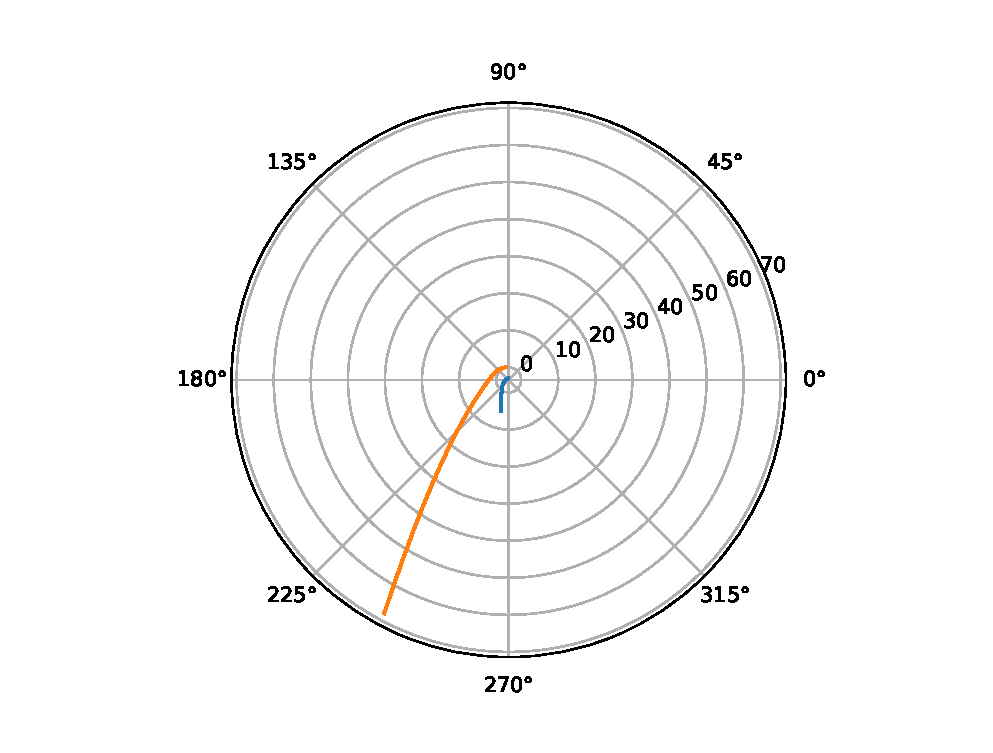
\includegraphics[width=\columnwidth]{./figs/ee18btech11002/ee18btech11002_1.eps}
\caption{Inverse Polar Plot}
\label{fig:ee18btech11002inverse_polar_plot}
\end{figure}


\end{enumerate}
